\begin{frame}{Difference of Two Means}
    What happens when we have two population means, but the data are not paired?
    \begin{itemize}
        \item The approach is similar to paired data.
        \item We will need a little bit more detail about each sample. 
        \item We will also develop a new standard error formula.
    \end{itemize}
\end{frame}

\begin{frame}{Examples}
    \begin{itemize}
        \item Do stem cells improve heart function?
        \item Is there a relationship between a pregnant person's smoking habits and birth weight?
        \item Is one version of an exam harder than another?
    \end{itemize}
\end{frame}

\begin{frame}{Confidence Interval for Difference of Means}
    Research question: Does treatment using embryonic stem cells (ESCs) help improve heart function following a heart attack?
    \begin{itemize}
        \item Tested in sheep post heart attack.
        \item 9 sheep assigned to treatment group (ESCs)
        \item 9 sheep assigned to control (no ESCs)
        \item Measured change in hearts' pumping capacity.
    \end{itemize}
\end{frame}

\begin{frame}{Confidence Intervals for Difference of Means}
    Summary statistics:
    \begin{table}[]
        \centering
        \begin{tabular}{cccc}
            \hline
                    & $n$ & $\bar{x}$ & $s$ \\
            \hline
            ESCs    & 9 & 3.50 & 5.17 \\
            control & 9 & -4.33 & 2.76 \\
            \hline
        \end{tabular}
    \end{table}
    \vspace{12pt}
    The point estimate for the difference of population means is the difference of the sample means.
\end{frame}

\begin{frame}{The t-Distribution for Difference of Means}
    To use a t-distribution, we require
    \begin{enumerate}
        \item Independence
        \begin{itemize}
            \item Within groups.
            \item Between groups
        \end{itemize}
        \item Normality
        \begin{itemize}
            \item Check each group separately.
        \end{itemize}
    \end{enumerate}
\end{frame}

\begin{frame}{The t-Distribution for Difference of Means}
    The standard error may now be computed as
    \[
        SE = \sqrt{\frac{\sigma_1^2}{n_1} + \frac{\sigma_2^2}{n_2}}
    \]
    
    \vspace{12pt}The degrees of freedom is calculated using a complex formula, but for this course you may use
    \[
        \min(n_1-1, n_2-1)
    \]
\end{frame}

\begin{frame}{Example: Sheep and ESCs}
    Can we use the t-distribution for inference about the point estimate $\bar{x}_{esc} - \bar{x}_{control} = 7.83$?
\end{frame}

\begin{frame}{Example: Sheep and ESCs}
    \begin{center}
        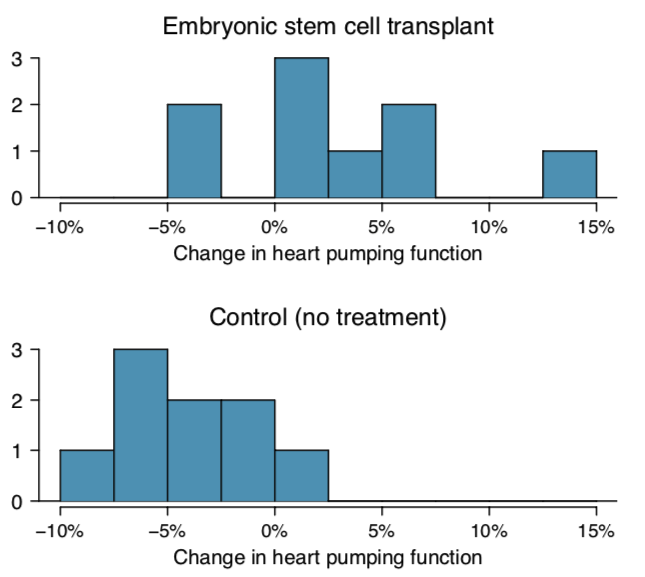
\includegraphics[scale=0.3]{images/escsheep.png}
    \end{center}
\end{frame}

\begin{frame}{Example: Sheep and ESCs}
    Calculate the standard error and degrees of freedom for the ESC research using the summary statistics: 
    \begin{table}[]
        \centering
        \begin{tabular}{cccc}
            \hline
                    & $n$ & $\bar{x}$ & $s$ \\
            \hline
            ESCs    & 9 & 3.50 & 5.17 \\
            control & 9 & -4.33 & 2.76 \\
            \hline
        \end{tabular}
    \end{table}
\end{frame}

\begin{frame}{Example: Sheep and ESCs}
    Calculate a 95\% confidence interval for the difference in heart pumping capacity between ESCs and the control.
\end{frame}

\begin{frame}{Statistical Inference Procedure}
    The details may change, but the general approach is always:
    \begin{enumerate}
        \item \textbf{Prepare.} Pick out critical contextual information and set up hypotheses.
        \item \textbf{Check} conditions.
        \item \textbf{Calculate} standard error and confidence interval/test statistic.
        \item \textbf{Conclude} based on context.
    \end{enumerate}
\end{frame}

\begin{frame}{Hypothesis Tests for Difference of Two Means}
    North Carolina births data:
    \begin{itemize}
        \item 150 mothers with newborns
        \item \texttt{weight}: weight of newborn
        \item \texttt{smoke}: mother's smoking habits during pregnancy (yes/no)
    \end{itemize}
    
    \vspace{12pt}Question: Do newborns from mothers who smoke have a different average birth weight than those from mothers who don't smoke?
\end{frame}

\begin{frame}{North Carolina Births Data}
    \begin{center}
        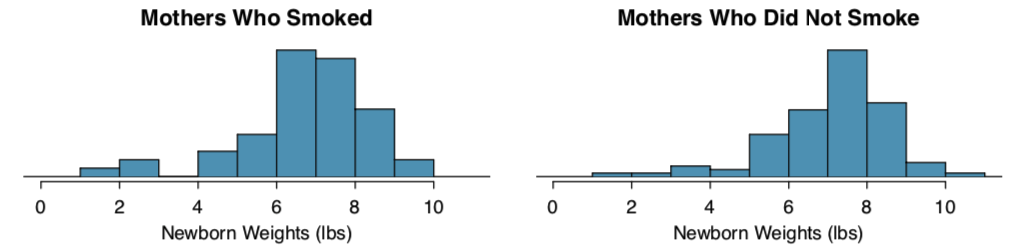
\includegraphics[scale=0.3]{images/twogrp_brthwt.png}
    \end{center}
    
    \begin{table}[]
        \centering
        \begin{tabular}{lrr}
        \hline
                    & smoker & nonsmoker \\
        \hline
        mean        & 6.78 & 7.18 \\
        std dev     & 1.43 & 1.60 \\
        sample size & 50 & 100 \\
        \hline
        \end{tabular}
    \end{table}
\end{frame}

\begin{frame}{North Carolina Births Data}
    \begin{itemize}
        \item<1-> Set up hypotheses for the birth weight and smoking data.
        \item<2-> Check conditions.
        \item<3-> Calculate the point estimate and standard error.
        \item<4-> Find the test statistic.
        \item<5-> Find the critical value.
        \item<6-> Draw conclusions.
    \end{itemize}
\end{frame}

\begin{frame}{North Carolina Births Data}
    The overall scientific conclusion is that smoking results in a lower birth weight. What happened?
\end{frame}

\begin{frame}{Case Study: Course Exams}
    We have two slight variations of the same exam, randomly assigned to students in a course.
    \begin{table}[]
        \centering
        \begin{tabular}{lrr}
        \hline
                    & Version A & Version B \\
        \hline
        $n$         & 30    & 27 \\
        $\bar{x}$   & 79.4  & 74.1 \\
        $s$         & 14  & 20 \\
        min         & 45    & 32 \\
        max         & 100    & 100 \\
        \hline
        \end{tabular}
    \end{table}
    Is there enough evidence to conclude that one version is more difficult (on average) than the other?
\end{frame}

\begin{frame}{Pooled Standard Deviation}
    Our standard error for two-sample means is
    \[
        SE = \sqrt{\frac{\sigma_1^2}{n_1} + \frac{\sigma_2^2}{n_2}}
    \]
    What if we have reason to believe that $\sigma_1=\sigma_2$?
\end{frame}

\begin{frame}{Pooled Standard Deviation}
    \begin{itemize}
        \item Sometimes two populations will have the same standard deviation.
        \item We might have a lot of existing data or a well-understood mechanism that justifies this.
        \item Sometimes we may also test equality of variances.
    \end{itemize}
\end{frame}

\begin{frame}{Pooled Standard Deviation}
    Here we can improve the t-distribution approach by using a pooled standard deviation (pooled variance):
    \[
        s^2_{\text{pooled}} = \frac{(n_1-1)s_1^2 + (n_2-1)s_2^2}{n_1+n_2-2}
    \]
\end{frame}

\begin{frame}{Pooled Standard Deviation}
    Then the standard error is
    \[
        SE \approx \sqrt{\frac{s^2_{\text{pooled}}}{n_1} + \frac{s^2_{\text{pooled}}}{n_2}}
    \]
    with degrees of freedom
    \[
        df = n_1 + n_2 - 2.
    \]
\end{frame}
